% \documentclass[preprint]{kcc}
\documentclass{kcc}


%%%%%%%%%%%%%%%%%%%%%%%%%%%%%%%%%%%%%%%%%%%%%%%
% include additional packages you need to use
%%%%%%%%%%%%%%%%%%%%%%%%%%%%%%%%%%%%%%%%%%%%%%%
% graphic, float package
\usepackage{graphicx}		% for setting images
\usepackage{float}			% for float objects
\usepackage{subfloat}		
\usepackage{subfigure}		% for adding several figures in a figure environment
\usepackage{lscape}			% for landscape type images or tables


\usepackage{enumitem}

% for compact section title spacing
% \usepackage[compact]{titlesec}


% mathmetical presentation
\usepackage{gensymb}
\usepackage{amsmath}
\usepackage{amssymb}
\usepackage{amsthm}
\usepackage{exscale}
\usepackage{textcomp}		% extra symbols


% for circled number
\newcommand{\cl}[1]{\textcircled{\scriptsize #1}}


% package for using algorithmic presentation
\usepackage{algorithmic}
\usepackage{algorithm}
% customize algorithmic environment
\renewcommand{\algorithmicrequire}{\makebox[40px]{\hfill\textbf{Input :}}}
\renewcommand{\algorithmicensure}{\makebox[40px]{\hfill\textbf{Output :}}}

% array and table presentation
\usepackage{array}
\usepackage{tabulary}
\usepackage{multirow}
\usepackage[table]{xcolor}
\usepackage{ctable}
\usepackage{booktabs}		% for typesetting tables at the level of publication		
							% do not use vertical rule
							
							\usepackage{times}
\usepackage{CJKutf8}
\usepackage{mathrsfs}
\usepackage{verbatim}
\usepackage{amsfonts}
\usepackage{xspace}
\usepackage{xcolor}
\usepackage{url}
\usepackage{balance}
\usepackage{booktabs}
\usepackage{multirow}
\usepackage{rotating}
\usepackage{fancyvrb}
\usepackage{lastpage}
\usepackage{alltt}
\usepackage{etoolbox}
\usepackage{cleveref} % After hyperref, listings
\usepackage{fancyhdr}
\usepackage{listings}

\usepackage{caption}


% set title, author, abstract
\title{매니코어 환경에서 PARSEC 벤치마크 ROI 확장성 분석}
\author{
}
\engtitle{An Analysis of ROI Scalability on PARSEC \\Benchmark for Many-core
System} \engauthor{
}
\abstract{
한국정보과학회는 정보과학에 관한 기술을 발전, 보급시키고 회원상호간의 친목을 
도모하기 위하여 1973년 3월 3일에 설립되었으며, 
정보통신부에 `사단법인 한국정보과학회'로 등록되었다.  
학회의 주요 활동은 
1) 컴퓨터 기술 및 이론에 관한 새로운 연구결과를 발표하는 기회를 제공하고, 
2) 국내의 컴퓨터 관련 기술 개발에 참여 하며, 
3) 국제적 학술 교류 및 협력 증진을 도모 하고, 
4) 회원 상호간의 친목을 증진시키는 것이다.
}


\begin{document}

\maketitle


\section{서 론}
학회는 설립 당시 500여 명의 회원으로 시작해서 지난 38년 동안 눈부신 발전을 거듭하여 
2011년 1월 현재 일반회원 30,080 여명, 특별회원 133개 기관, 단체회원 269개 기관이 등록된 대규모 학회로 성장하였다. 
본 학회는 1977년에 IFIP(International Federation for Information Processing)에 정회원으로 가입했고, 
ACM.IEEE Computer Society.SEARCC(The South East Asia Regional Computer Conference)와의 협력관계를 맺음으로써 
국제 학술교류 및 협력을 강화하고 있으며, 또한 IPSJ(일본정보처리학회)와도 유대관계를 유지하고 있다.


\section{관련 연구}


\section{실험 환경}

\begin{figure}[h]
  \begin{center}
     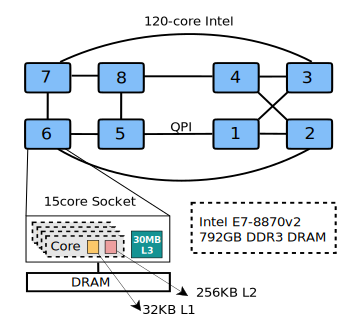
\includegraphics[width=0.3\textwidth]{fig/xeon}
  \end{center}
  \caption{Test-bed Intel Xeon architecture.}
  \label{fig:basic}
\end{figure}


\begin{table}[h!]
  \centering
  \small
  \begin{tabular}{l c c c c} \toprule
    워크로드 & 설명 & 입력 데이터\\
    \midrule
    Word Count & 10G & 4G & none & text \\ 
    Naive Basian & 10G & 4G & none & text\\
    Grep & 30G & 4G &  & text\\
    K-means & 4G & 4G & k=8 & graph\\
    \bottomrule
  \end{tabular}
  
  \begin{tabular}{l l l l l} \toprule
    JVM & Spark & OS & Distribution\\
    \midrule
    Openjdk 1.8.0\_91 & 1.3.1 & 1.2.1 & Linux 4.5-rc6 & Ubuntu 14.04\\ 
    \bottomrule
  \end{tabular}
  \caption{System information and configuration values.}
  \label{tab:memuse}
\end{table}

\section{확장성 실험}


\section{PARSEC CPU 사용량 분석}


\section{PARSEC 메모리 사용량 분석}


\section{결론 및 향후 연구}

\bibliographystyle{ieeetr}
\bibliography{ref}

\end{document}
